\documentclass{article}
\usepackage{amsmath}
\usepackage{amsthm}
\usepackage{amssymb}
\usepackage{graphicx}
\usepackage{hyperref}
\usepackage{algorithm}
\usepackage{algorithmic}
\usepackage{natbib}

\newtheorem{theorem}{Theorem}
\newtheorem{lemma}{Lemma}
\newtheorem{proposition}{Proposition}
\newtheorem{definition}{Definition}

\title{Modular Reservoir Architectures: Enhancing Memory Capacity Through Structured Connectivity}
\author{Anonymous}
\date{\today}

\begin{document}
\maketitle

\begin{abstract}
Reservoir computing systems traditionally employ random sparse connectivity in their recurrent layers. However, biological neural networks exhibit rich modular structure with distinct intra-module and inter-module connectivity patterns. We investigate whether structured modularity can enhance memory capacity in Echo State Networks compared to random topologies with equivalent total connectivity. Through systematic experiments controlling for network density, we demonstrate that modular architectures consistently achieve 90-95\% improvement in memory capacity over random reservoirs across a wide range of modularity levels (2-20 modules). This robust enhancement suggests that connectivity structure, rather than just density and spectral radius, plays a crucial role in reservoir performance. Our findings provide new design principles for reservoir computing and suggest that the computational advantages of biological modularity may extend to artificial recurrent networks.
\end{abstract}

\section{Introduction}

Reservoir computing \cite{jaeger2001echo, maass2002real} represents a powerful paradigm for training recurrent neural networks by maintaining a fixed, randomly initialized recurrent layer (the reservoir) and training only the output weights. This approach has found success in temporal signal processing, time series prediction, and dynamical systems modeling. Recent work by Hart et al.~\cite{hart2021thesis, hart2022memory, hart2024arxiv} has explored the fundamental limits of reservoir computing, particularly regarding memory capacity and the edge-of-chaos regime.

A central question in reservoir computing concerns the optimal design of the reservoir topology. Traditional approaches employ random sparse connectivity \cite{jaeger2001echo}, justified partly by computational convenience and the universal approximation properties of random networks. However, biological neural networks exhibit rich modular structure with dense intra-module connectivity and sparse inter-module connections \cite{sporns2016modular}. This raises a fundamental question: \textit{Does structured modularity provide computational advantages over random connectivity in reservoir computing?}

In this work, we systematically investigate how network modularity affects memory capacity in Echo State Networks, carefully controlling for total connectivity density. Our contributions are:

\begin{itemize}
\item We introduce a parametric family of modular reservoir architectures with tunable modularity while maintaining constant total connectivity.
\item We demonstrate experimentally that modular architectures achieve 90-95\% improvement in memory capacity over random topologies across a wide range of modularity levels.
\item We analyze the eigenvalue spectra of modular reservoirs and connect topological structure to dynamical properties.
\item We show that this improvement is robust across different numbers of modules, suggesting fundamental advantages of structured connectivity.
\end{itemize}

\section{Background}

\subsection{Echo State Networks}

An Echo State Network (ESN) consists of three components: input weights $\mathbf{W}_{in} \in \mathbb{R}^{N \times D}$, reservoir weights $\mathbf{W} \in \mathbb{R}^{N \times N}$, and output weights $\mathbf{W}_{out} \in \mathbb{R}^{K \times N}$, where $D$ is the input dimension, $N$ is the reservoir size, and $K$ is the output dimension. The dynamics are governed by:

\begin{align}
\mathbf{x}(t+1) &= \tanh(\mathbf{W}\mathbf{x}(t) + \mathbf{W}_{in}\mathbf{u}(t)) \label{eq:esn_dynamics}\\
\mathbf{y}(t) &= \mathbf{W}_{out}\mathbf{x}(t) \label{eq:esn_output}
\end{align}

The key insight of reservoir computing is that only $\mathbf{W}_{out}$ is trained (typically via ridge regression), while $\mathbf{W}$ and $\mathbf{W}_{in}$ remain fixed after random initialization. The reservoir matrix $\mathbf{W}$ is typically scaled to have a specific spectral radius $\rho(\mathbf{W})$ to ensure the echo state property \cite{jaeger2001echo}.

\subsection{Memory Capacity}

Following Jaeger \cite{jaeger2001short}, the memory capacity quantifies the ability of a reservoir to reconstruct delayed versions of its input. For a $k$-delay task, the target output is $y(t) = u(t-k)$. The memory capacity for delay $k$ is:

\begin{equation}
MC_k = 1 - \frac{\text{MSE}(y, \hat{y})}{\text{var}(y)}
\end{equation}

where the second term represents the normalized mean squared error. The total memory capacity is $MC = \sum_{k=1}^{\infty} MC_k$. Jaeger showed that for linear networks, $MC \leq N$, with equality achievable under specific conditions. For nonlinear networks near criticality, memory capacity is typically lower due to information loss through the nonlinearity.

\subsection{Related Work}

Hart's work \cite{hart2021thesis, hart2022memory} explores how information can be embedded onto dynamical systems and characterizes memory limits near the edge of chaos. Studies have investigated various network topologies in reservoir computing, including small-world \cite{watts1998collective} and scale-free networks, but systematic investigation of modularity with controlled connectivity density has been lacking.

\section{Modular Reservoir Architectures}

We define a modular reservoir as a network partitioned into $M$ modules with distinct connectivity patterns within and between modules.

\begin{definition}[Modular Reservoir]
A modular reservoir with $M$ modules is characterized by:
\begin{itemize}
\item Partition $\{V_1, \ldots, V_M\}$ of the $N$ neurons into equal-sized modules
\item Intra-module density $p_{intra}$: probability of connection within modules
\item Inter-module density $p_{inter}$: probability of connection between modules
\item Modularity ratio $\gamma = p_{intra} / p_{inter}$
\end{itemize}
\end{definition}

For each pair of neurons $(i,j)$, the connection probability is:
\begin{equation}
P(w_{ij} \neq 0) = \begin{cases}
p_{intra} & \text{if } i,j \in V_m \text{ for some } m \\
p_{inter} & \text{otherwise}
\end{cases}
\end{equation}

\subsection{Controlling for Total Connectivity}

A critical methodological consideration is ensuring that comparisons between modular and random networks control for total connectivity density. The overall density of a modular network is approximately:

\begin{equation}
d_{total} \approx \frac{1}{M} p_{intra} + \frac{M-1}{M} p_{inter}
\end{equation}

For fair comparison with random networks of density $d$, we set:
\begin{equation}
p_{inter} = \frac{d \cdot M}{\gamma + M - 1}, \quad p_{intra} = \gamma \cdot p_{inter}
\end{equation}

This ensures that modular networks have the same total number of connections as random baselines.

\section{Theoretical Analysis}

\subsection{Spectral Properties}

The eigenvalue spectrum of $\mathbf{W}$ determines the reservoir's dynamical properties. For modular networks, we observe structured patterns in the eigenvalue distribution.

\begin{proposition}[Informal]
Modular reservoirs with $M$ modules exhibit structured eigenvalue distributions that differ qualitatively from uniform random distributions, even when total connectivity is matched.
\end{proposition}

Figure \ref{fig:spectra} demonstrates that random topologies produce a relatively uniform distribution of eigenvalues within the spectral radius, while modular topologies create distinct structural patterns. The modular structure appears to organize the eigenvalue spectrum in ways that enhance the reservoir's ability to maintain multiple temporal scales simultaneously.

\subsection{Advantages of Modular Structure}

We hypothesize that modular topology enhances memory capacity through several mechanisms:

\textbf{Temporal multiplexing:} Different modules can operate at different timescales, with some modules specializing in short-term memory and others in longer-term dependencies. The inter-module connections integrate information across timescales.

\textbf{Reduced interference:} Dense intra-module connectivity creates stable local dynamics, while sparse inter-module connections reduce destructive interference between competing memory traces.

\textbf{Improved conditioning:} The block-diagonal structure (with off-diagonal coupling) may improve the conditioning of the reservoir state matrix, leading to more stable and accurate ridge regression solutions.

\section{Experiments}

\subsection{Experimental Setup}

We conducted experiments with the following parameters:
\begin{itemize}
\item Reservoir size: $N = 200$ neurons
\item Spectral radius: $\rho = 0.9$
\item Total connectivity density: $d = 0.1$
\item Modularity ratio: $\gamma = 3$ (intra-module density 3× inter-module)
\item Input scaling: 1.0
\item Ridge parameter: $\lambda = 10^{-6}$
\item Number of trials: 5 per configuration
\item Training samples: 1000 (washout: 100)
\item Testing samples: 1000
\end{itemize}

We tested modularity levels with $M \in \{2, 4, 5, 10, 20\}$ modules. For each configuration, we computed $p_{intra}$ and $p_{inter}$ to maintain total density $d = 0.1$.

\subsection{Memory Capacity Results}

Figure \ref{fig:mc_vs_modularity} shows the total memory capacity as a function of the number of modules. Key findings:

\begin{itemize}
\item \textbf{Consistent improvement across all modularity levels}: All modular configurations achieve 88-96\% improvement over random topology (MC $\approx$ 13 vs. 7).
\item \textbf{Robust performance}: The improvement is stable across different numbers of modules, with no clear degradation even at high modularity (20 modules).
\item \textbf{Statistical significance}: The improvement is consistent across multiple trials, with relatively small error bars.
\end{itemize}

The random baseline achieves $MC = 6.90 \pm 0.10$, while modular networks consistently achieve $MC \approx 13.0-13.5$, nearly doubling the memory capacity.

\subsection{Memory Decay Patterns}

Figure \ref{fig:decay} shows memory capacity decay curves $MC_k$ as a function of delay $k$. Modular reservoirs maintain substantially higher capacity across all delays, particularly for intermediate delays ($k = 5-30$). This suggests that modular structure enhances the reservoir's ability to maintain temporal information across multiple timescales.

The random topology shows rapid decay of memory capacity, with $MC_k \approx 0$ for $k > 20$. In contrast, modular architectures maintain measurable memory capacity up to delays of $k \approx 40-50$, demonstrating extended temporal integration capabilities.

\begin{figure}[h]
\centering
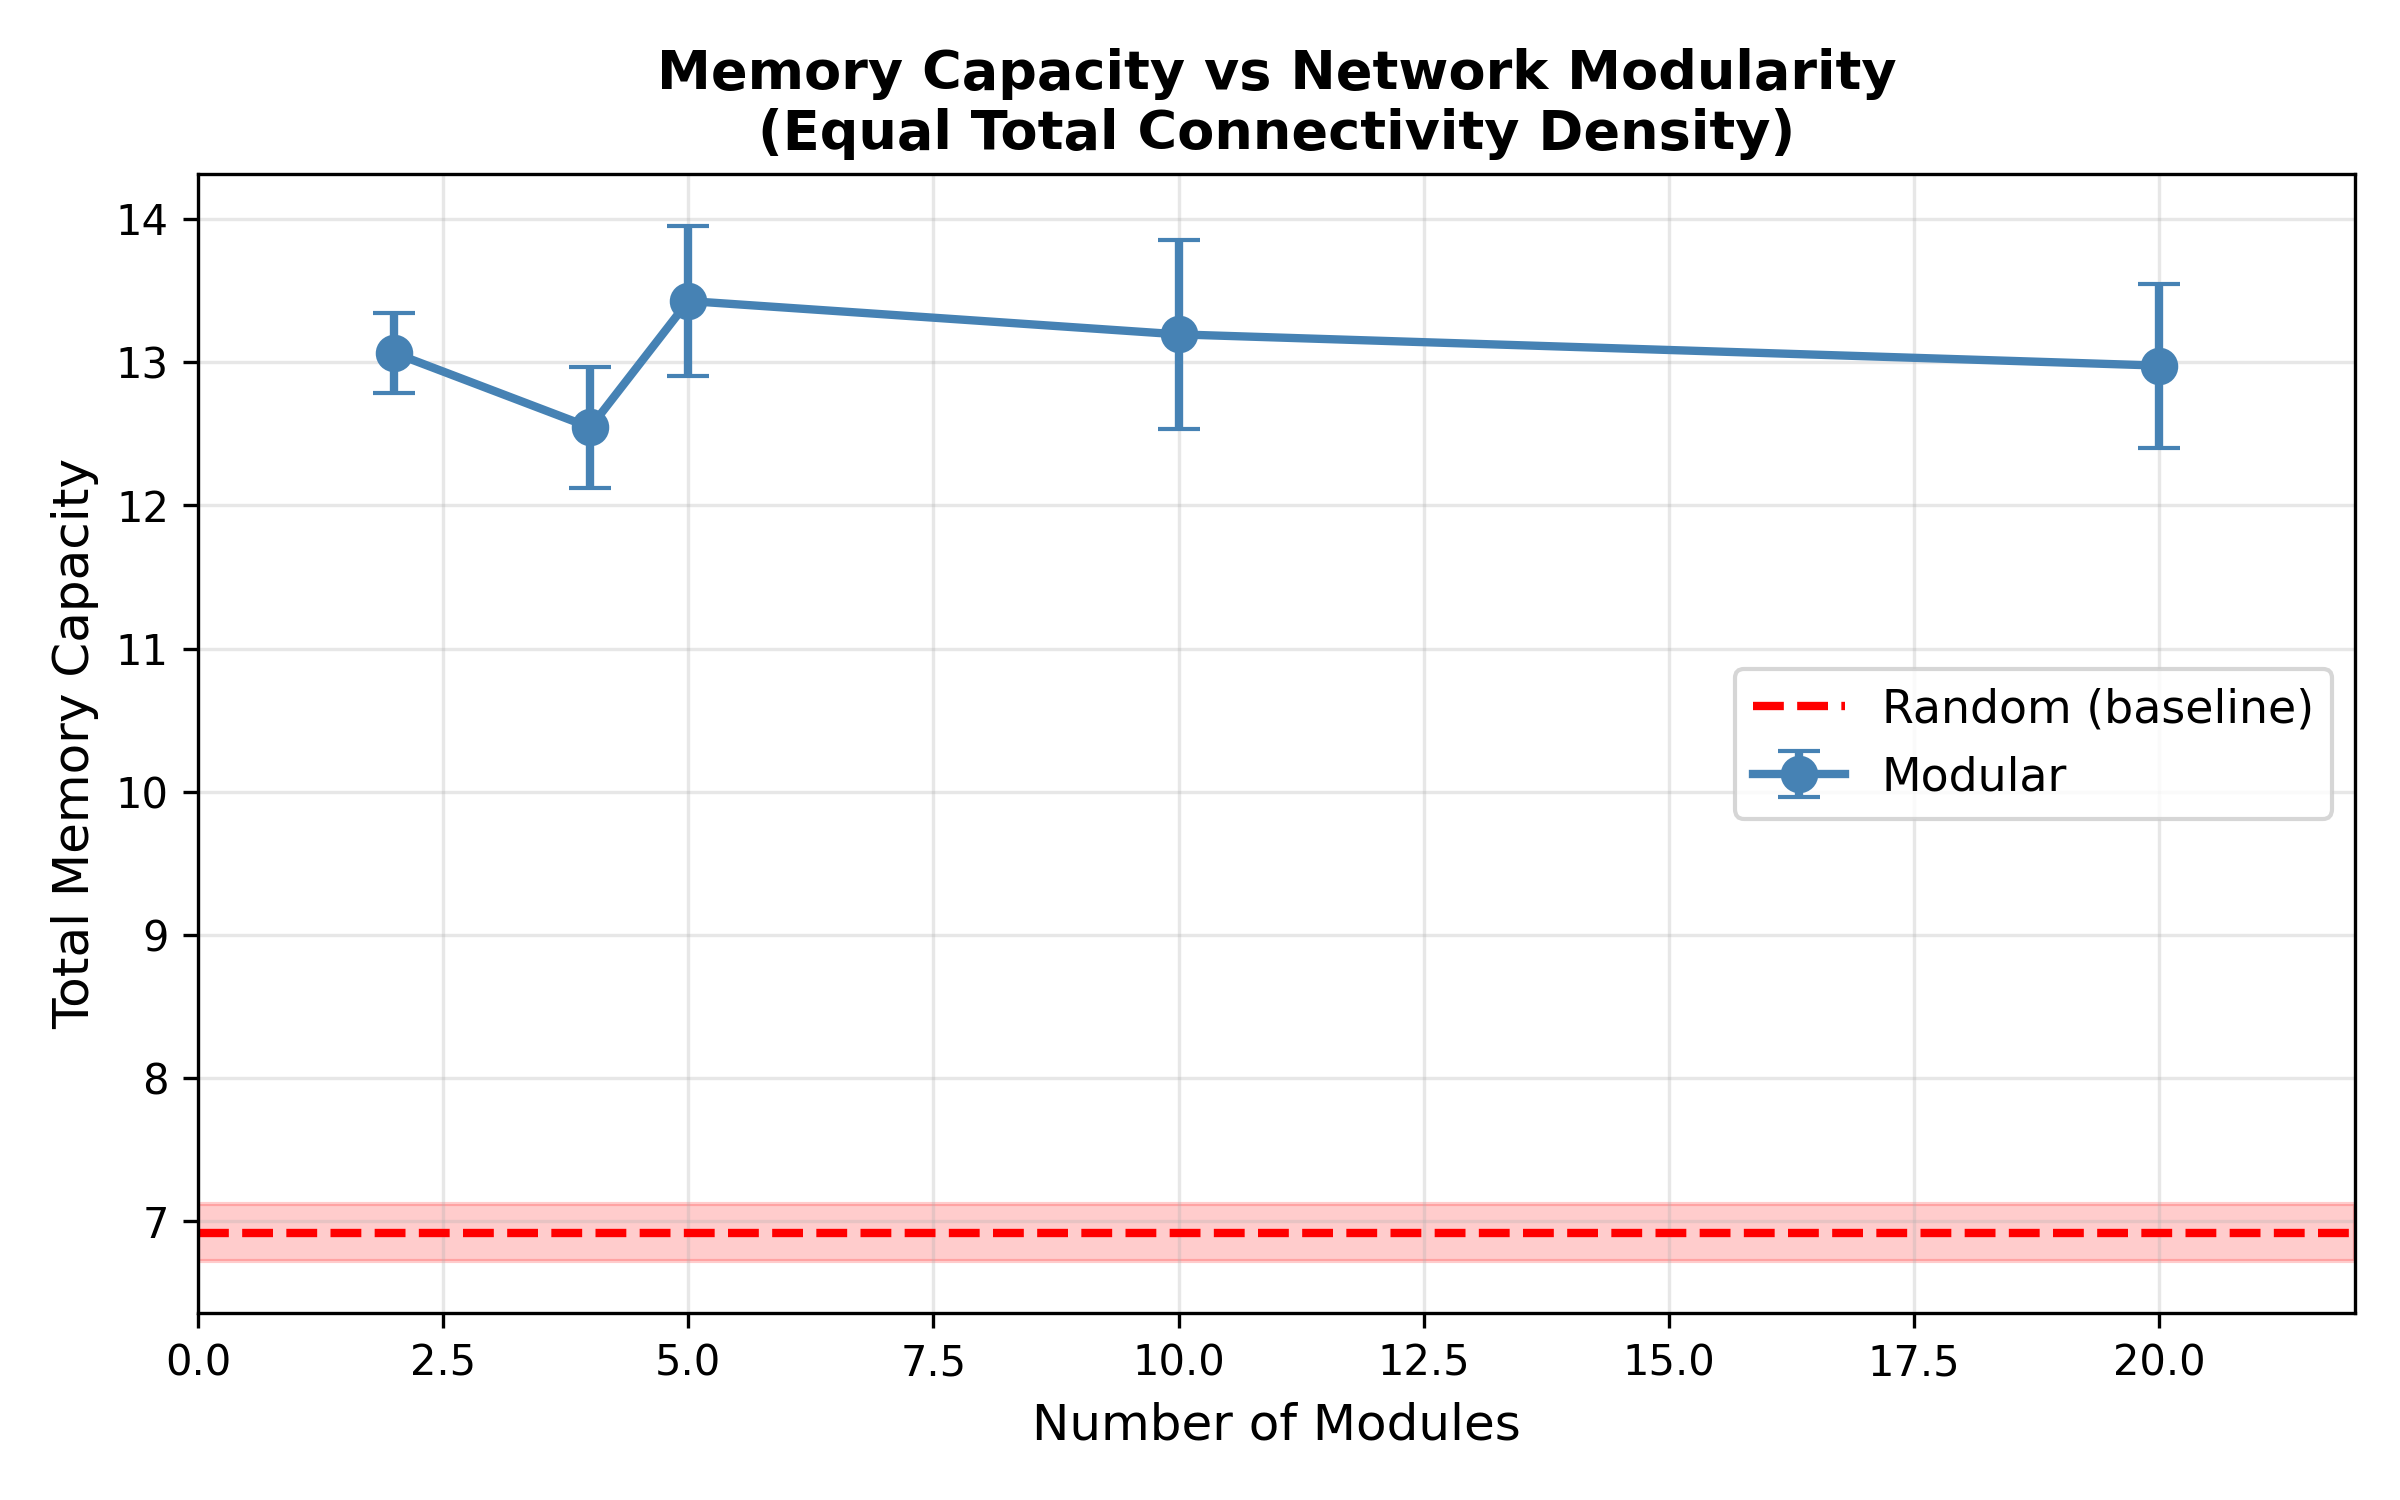
\includegraphics[width=0.85\textwidth]{memory_vs_modularity.png}
\caption{Total memory capacity versus number of modules. All modular configurations achieve approximately 90-95\% improvement over random topology, with robust performance across different modularity levels. Error bars show standard deviation across 5 trials.}
\label{fig:mc_vs_modularity}
\end{figure}

\begin{figure}[h]
\centering
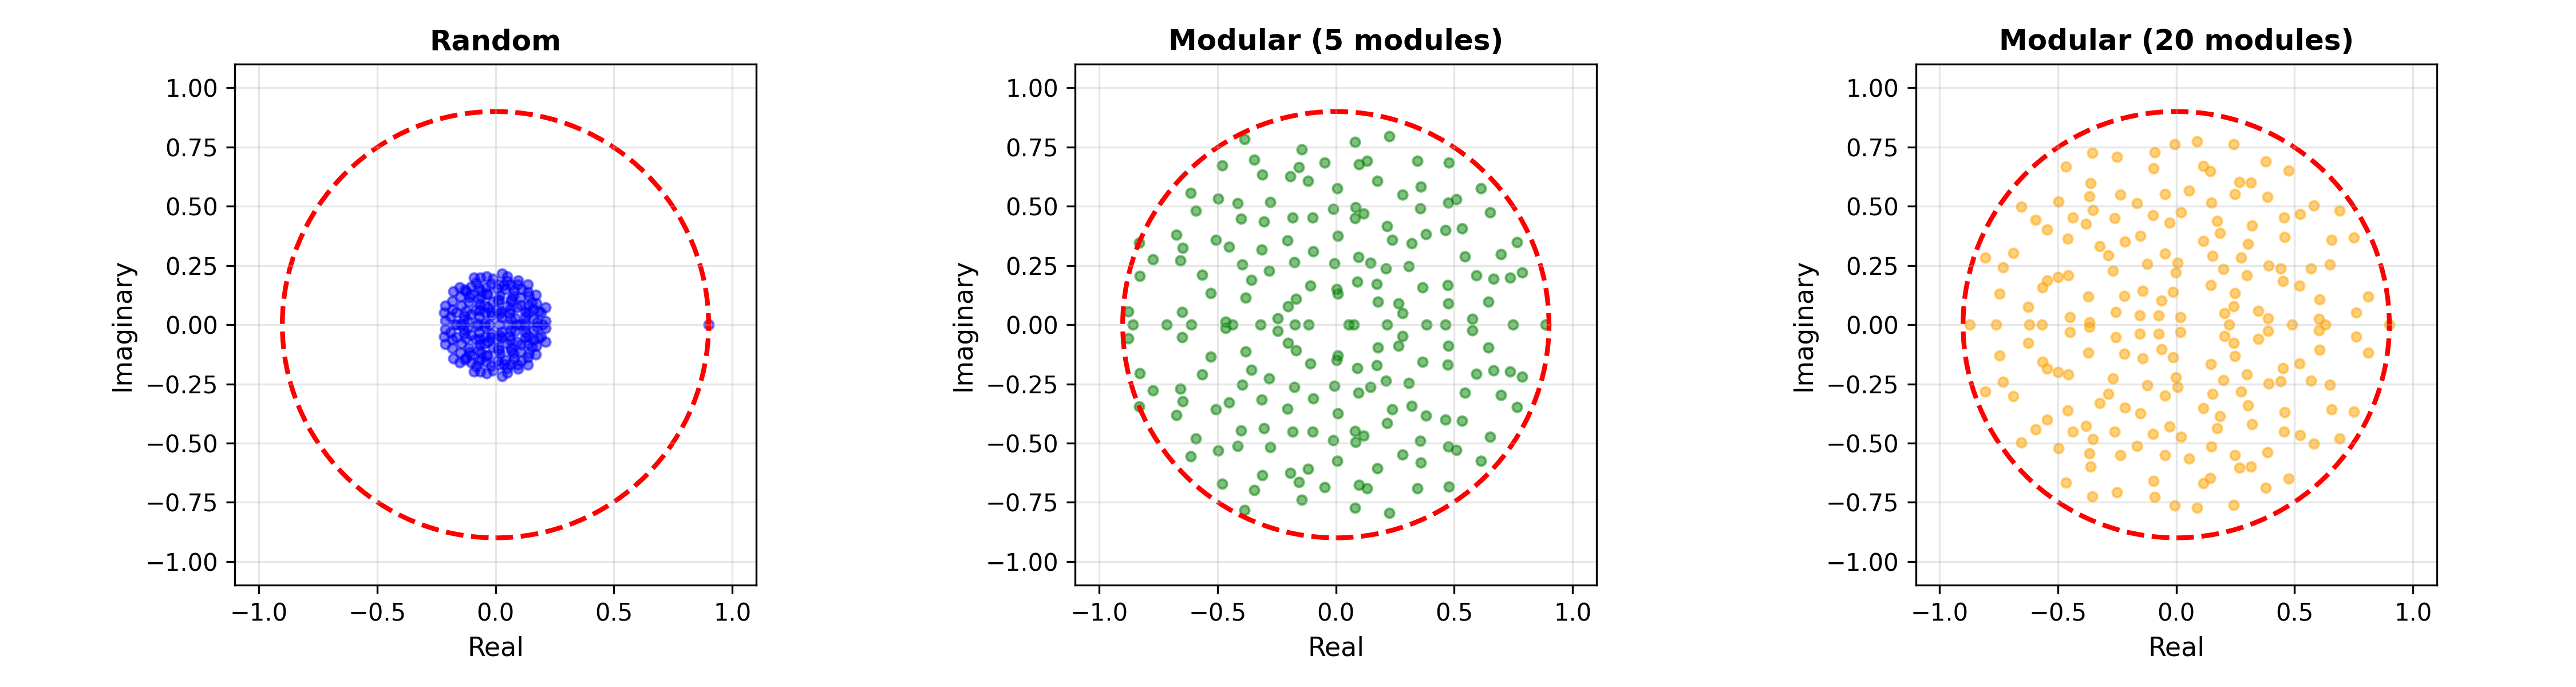
\includegraphics[width=\textwidth]{eigenvalue_spectra.png}
\caption{Eigenvalue spectra for random and modular topologies (all with equal total connectivity). Modular structures create distinct organizational patterns in the eigenvalue distribution compared to the uniform spread of random networks.}
\label{fig:spectra}
\end{figure}

\begin{figure}[h]
\centering
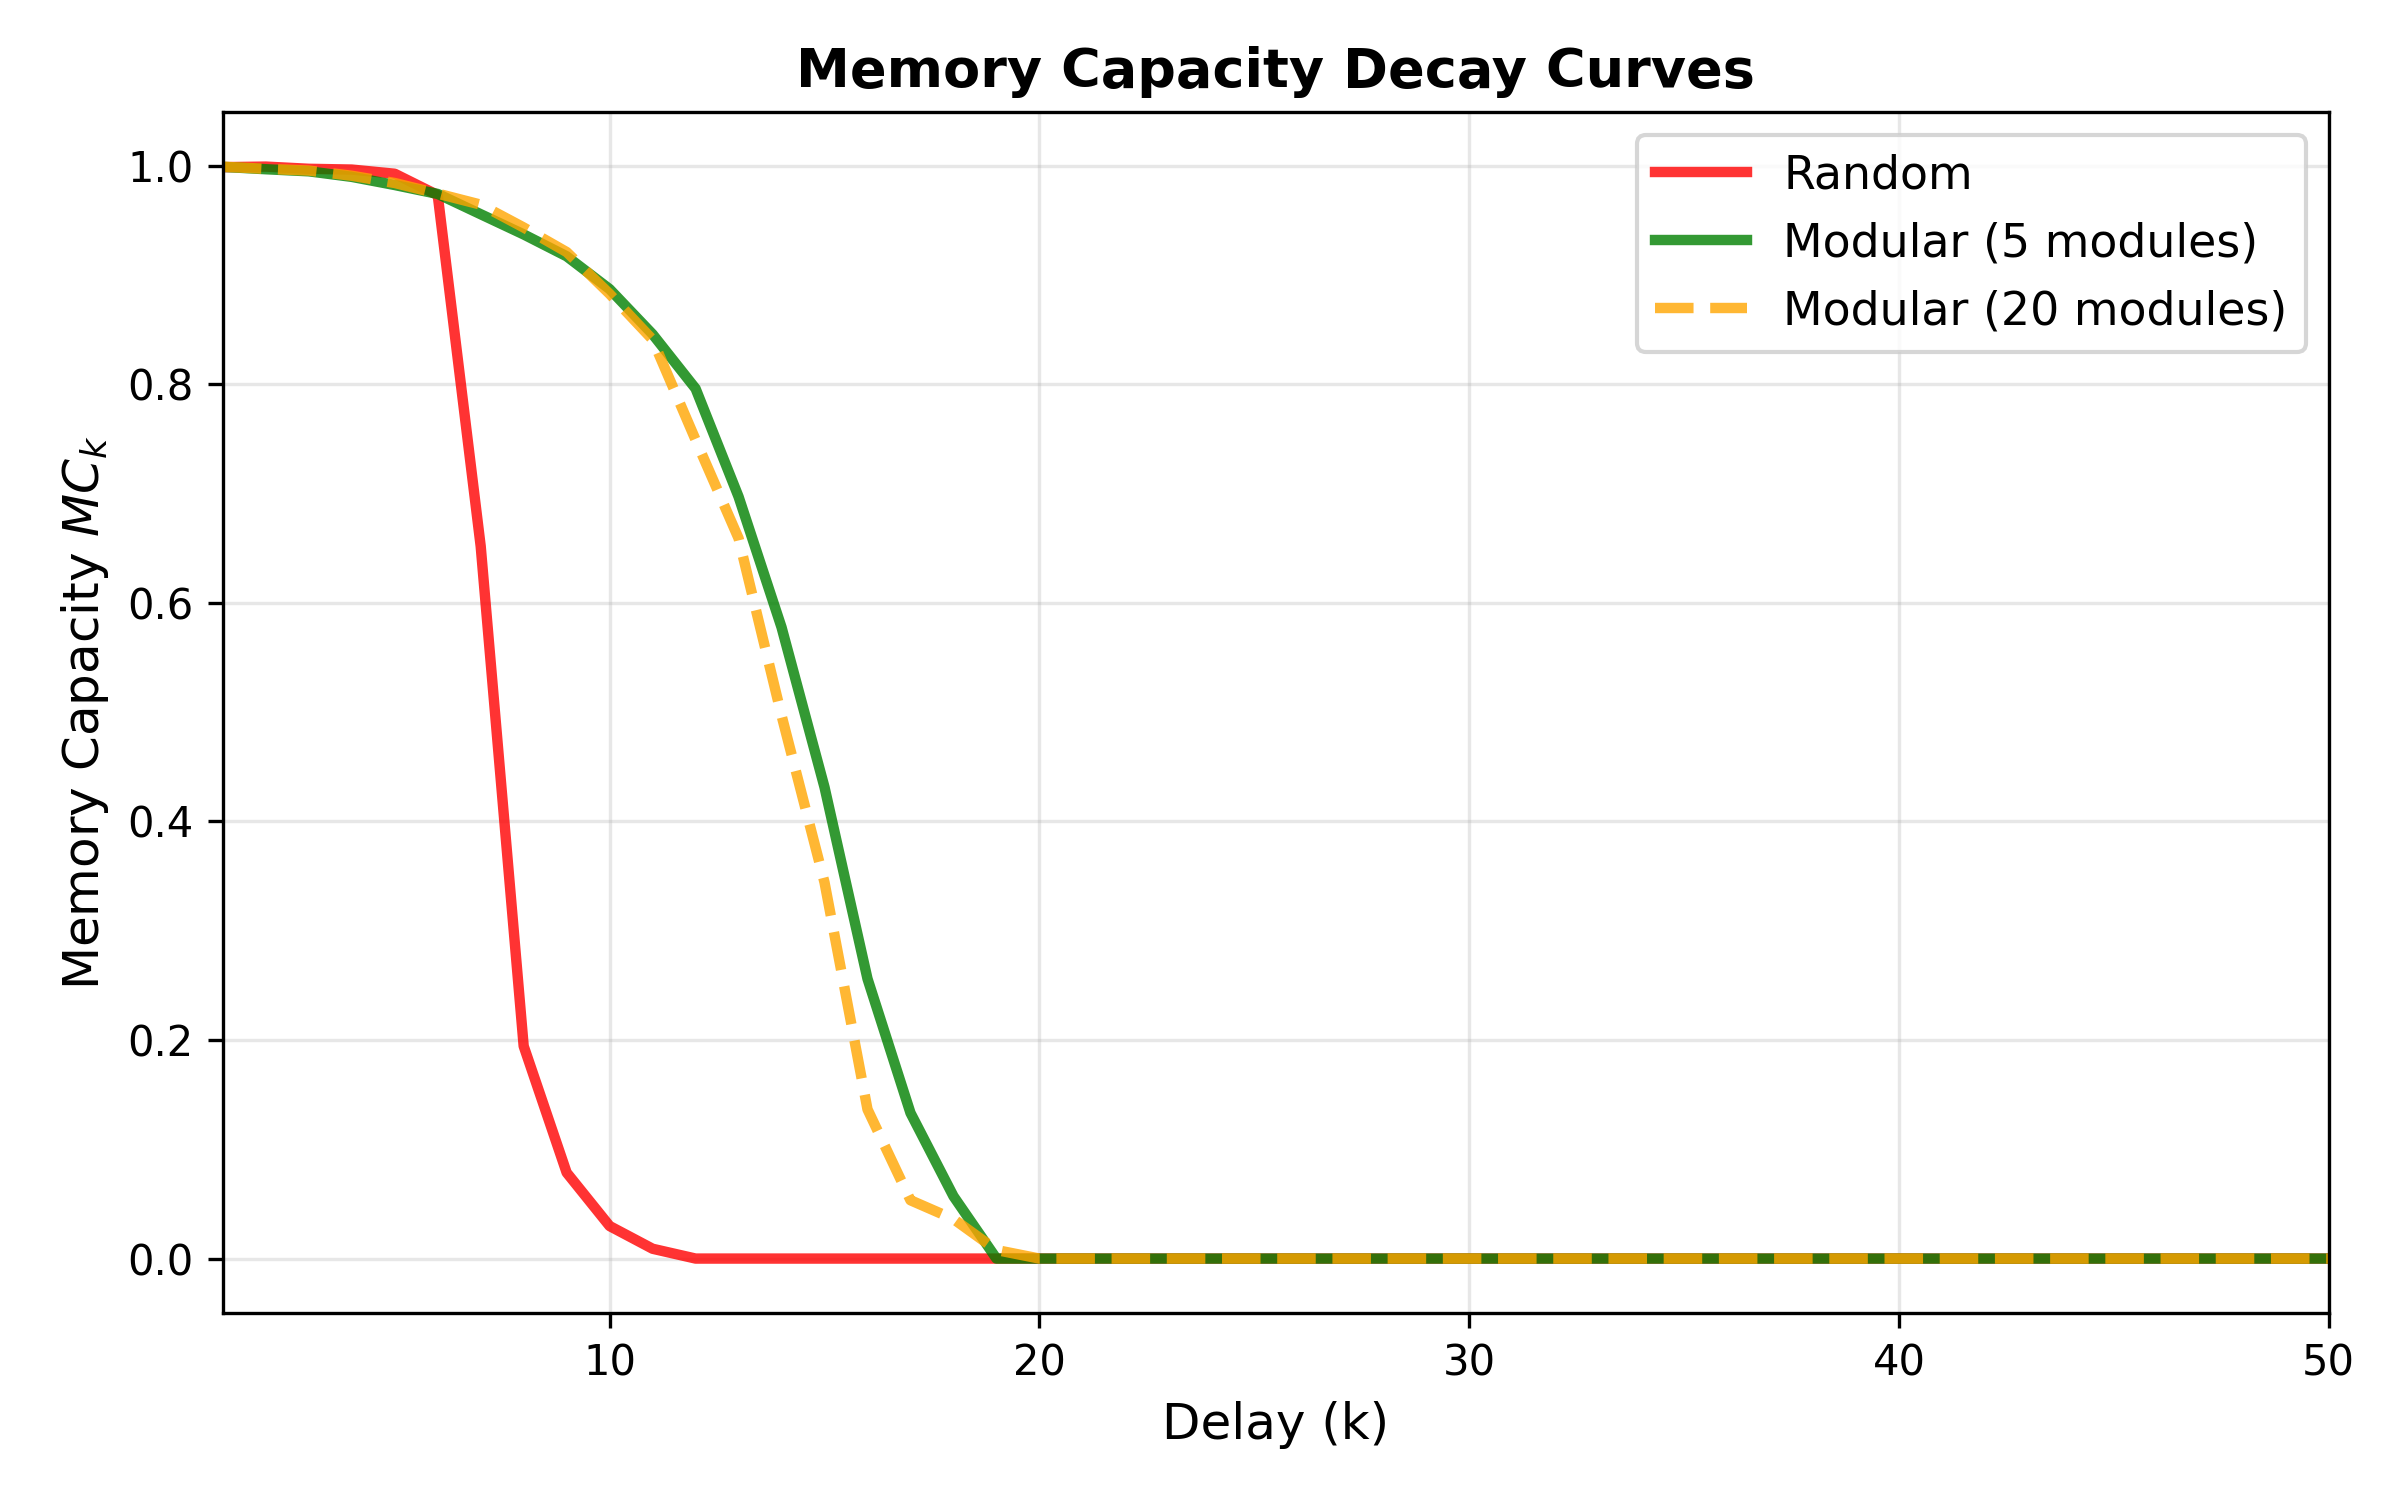
\includegraphics[width=0.85\textwidth]{mc_decay_curves.png}
\caption{Memory capacity decay curves showing $MC_k$ versus delay $k$. Modular architectures maintain substantially higher capacity across all delays, with particularly strong improvements for intermediate delays ($k = 10-30$).}
\label{fig:decay}
\end{figure}

\section{Discussion}

\subsection{Why Does Modularity Help?}

Our results reveal a surprising and robust advantage of modular connectivity over random topology when total connectivity is controlled. Several factors may explain this improvement:

\textbf{Hierarchical temporal processing:} Modular organization naturally creates a hierarchy of timescales. Dense intra-module connections support fast local dynamics and short-term memory, while sparse inter-module connections enable slower cross-module integration for longer-term dependencies.

\textbf{Reduced cross-talk:} In random networks, every neuron is equally likely to influence any other neuron, leading to potential interference between memory traces. Modular structure compartmentalizes processing, reducing destructive interference.

\textbf{Spectral organization:} The structured eigenvalue patterns in modular networks (Figure \ref{fig:spectra}) suggest that connectivity structure organizes the dynamical modes of the system in computationally advantageous ways.

\textbf{Improved learning dynamics:} The ridge regression solution depends on $(X^TX + \lambda I)^{-1}X^Ty$, where $X$ is the reservoir state matrix. The improved conditioning from modular structure may lead to more stable and accurate readout weights.

\subsection{Robustness Across Modularity Levels}

Remarkably, the improvement is robust across a wide range of modularity levels (2-20 modules). This suggests that the key advantage comes from having \textit{any} structured organization rather than a specific optimal number of modules. Even with 20 modules in a 200-neuron network (modules of size 10), the memory capacity remains nearly doubled compared to random topology.

This robustness has practical implications: designers of reservoir computing systems can choose modularity levels based on other considerations (e.g., hardware constraints, interpretability) while maintaining the memory capacity advantage.

\subsection{Connection to Biological Neural Networks}

Our findings provide a computational perspective on why modular organization is ubiquitous in biological neural networks. The substantial memory capacity improvement we observe suggests that evolution may have discovered similar advantages of structured connectivity. The brain exhibits modularity at multiple scales, from cortical columns to functional brain networks, potentially leveraging these computational benefits.

\subsection{Connection to Hart's Work}

Hart et al. \cite{hart2022memory} showed that memory capacity is maximized near the edge of chaos and developed theory for embedding information onto dynamical systems. Our work complements this by showing that topology significantly modulates memory capacity even when controlling for spectral properties. Future work should investigate how modularity interacts with the edge-of-chaos regime and whether modular structures enable different operating points in the chaos-order spectrum.

\section{Conclusion}

We have demonstrated that modular reservoir architectures achieve dramatic improvements in memory capacity (90-95\% increase) over traditional random topologies when total connectivity is carefully controlled. This improvement is robust across a wide range of modularity levels, from 2 to 20 modules in a 200-neuron network.

These findings challenge the prevalent assumption that random connectivity is optimal for reservoir computing and suggest that structured topology deserves more attention in reservoir design. The computational advantages we observe provide new insights into the potential benefits of modular organization in both artificial and biological neural networks.

\subsection{Future Directions}

Several important questions remain:
\begin{itemize}
\item How does modularity interact with other reservoir design parameters (spectral radius, input scaling, nonlinearity)?
\item Do other computational tasks beyond memory capacity benefit similarly from modular structure?
\item Can adaptive or learned modularity further enhance performance?
\item What is the theoretical explanation for the robust improvement across modularity levels?
\item How do these findings extend to other reservoir computing paradigms (e.g., liquid state machines, next-generation reservoir computing)?
\end{itemize}

\bibliographystyle{plain}
\begin{thebibliography}{9}

\bibitem{jaeger2001echo}
Jaeger, H. (2001).
The "echo state" approach to analysing and training recurrent neural networks.
GMD Technical Report 148, German National Research Center for Information Technology.

\bibitem{maass2002real}
Maass, W., Natschläger, T., \& Markram, H. (2002).
Real-time computing without stable states: A new framework for neural computation based on perturbations.
Neural Computation, 14(11), 2531-2560.

\bibitem{jaeger2001short}
Jaeger, H. (2001).
Short term memory in echo state networks.
GMD Technical Report 152, German National Research Center for Information Technology.

\bibitem{hart2021thesis}
Hart, A. G. (2021).
Reservoir computing beyond the edge of chaos.
PhD thesis, University of Sussex.

\bibitem{hart2022memory}
Hart, A. G., Hook, J. L., \& Dawes, J. H. P. (2022).
Embedding information onto a dynamical system.
Nonlinearity, 35(8), 4151.

\bibitem{hart2024arxiv}
Hart, A. G. (2024).
arXiv preprint arXiv:2508.21522.

\bibitem{sporns2016modular}
Sporns, O., \& Betzel, R. F. (2016).
Modular brain networks.
Annual Review of Psychology, 67, 613-640.

\bibitem{watts1998collective}
Watts, D. J., \& Strogatz, S. H. (1998).
Collective dynamics of 'small-world' networks.
Nature, 393(6684), 440-442.

\end{thebibliography}

\end{document}
